\documentclass[12pt]{article}
\usepackage[paper=a4paper,left=30mm,right=30mm,top=35mm,bottom =35mm]{geometry}
\usepackage[utf8]{inputenc}
\usepackage[T1]{fontenc}
\usepackage{stmaryrd}
\usepackage{setspace}
\usepackage{mathrsfs}
\usepackage[ngerman]{babel}
\usepackage{amssymb}
\usepackage{amsmath}
\usepackage{fancyhdr}
\usepackage[dvips,unicode,colorlinks,linkcolor=black]{hyperref} 
\usepackage{graphicx}
\usepackage{float}
\usepackage{listings}

\pagestyle{fancy}
\lfoot{}
\rfoot{Paul Kremser, Tobias Grussenmeyer}
\cfoot{\thepage}
\fancyhead[L]{FPI Versuch: Faraday- und Pockels-Effekt}
\renewcommand{\headrulewidth}{0.6pt}
\renewcommand{\footrulewidth}{0.6pt}
\setlength{\headheight}{16pt}
\setlength{\parindent}{0pt}
% Für die Wahl der Schriftart
\newcommand{\changefont}[3]{
\fontfamily{#1} \fontseries{#2} \fontshape{#3} \selectfont}

\lstset{
	basicstyle=\ttfamily\scriptsize\mdseries,
	keywordstyle=\bfseries\color{black},
	identifierstyle=,
	commentstyle=\color{black},	
	stringstyle=\itshape\color{black},
	numbers=left,
	numberstyle=\tiny,
	stepnumber=1,
	breaklines=true,
	frame=none,
	showstringspaces=false,
	tabsize=4,
	backgroundcolor=\color{white},
	captionpos=b,
	float=htbp,
	frame=tlrb
}

\begin{document}
% keine Hurenkinder und Schusterjungen
\clubpenalty = 10000
\widowpenalty = 10000 
\displaywidowpenalty = 10000

\onehalfspacing
% Schriftart
\changefont{ptm}{m}{n} 

\begin{titlepage}
\author{Paul Kremser, Tobias Grussenmeyer}
\title{Versuch: Faraday- und Pockels-Effekt}
\date{Versuchsdurchführung: 29. Oktober 2009} 
\maketitle
\thispagestyle{empty}
\end{titlepage}


\tableofcontents
\thispagestyle{empty}
\newpage
\pagenumbering{arabic}
\section{Überblick}
Faraday- und Pockelseffekt stellen Möglichkeiten dar einen Lichtstrahl zu beeinflussen. Insbesondere lässt sich die Intensität verändern. Dies wird in vielen technischen Anwendungen ausgenutzt z.B. LCD-Display. In diesem Versuch sollen der Pockelseffekt anhand von Ammoniumdihydrogenphosphat Kristallen und der Faradayeffekt mittels Schwerflintglas untersucht werden.

\section{Aufgabestellung}
\begin{itemize}


 \item Messung des elektrooptischen Koeffizienten beim Pockelseffekt mittels:
\begin{itemize}
 \item Sägezahnmethode
 \item Modulierter Gleichspannung
\end{itemize}

 \item Messung der Verdetkonstanten von Schwerflintglas bei der Natriumlinie.
 
\end{itemize}
\section{Theoretische Grundlagen}

\subsection{Pockelseffekt}

Bei manchen Kristallen oder Flüssigkeiten ändert sich der Brechungsindex, bezüglich einer bestimmten Richtung, durch anlegen eines elektrischen Feldes. Dieses Phänomen wird als elektrooptischer Effekt bezeichnet. Beim Pockelseffekt hängt die Phasenverschiebung zwischen zwei bestimmten Polarisationskomponenten des hindurchtretenden Lichtes linear von der angelegten Spannung ab. Der Pockelseffekt wird deshalb auch linearer optischer Effekt genannt.\\

Physikalisch wird der Pockelseffekt durch die Doppelbrechung erklärt.
Als \textbf{Doppelbrechung} wird die Eigenschaft von anisotropen Materialien bezeichnet, ein Lichtbündel in zwei senkrecht zueinander polarisierte Teilbündel aufzuspalten. Die Ursache dieses Effekts liegt in unterschiedlichen Brechzahlen in Abhängigkeit von der Ausbreitungsrichtung und Polarisation des Lichtes.

Solche optisch anisotropen Materialien zeichnen sich dadurch aus, dass sie verschiedene Brechzahlen für verschiedene Polarisationen und Richtungen des eingestrahlten Lichtes aufweisen. Dies lässt sich mit dem Brechzahl-Ellipsoid darstellen. Dieses Ellipsoid kann ein Rotationsellipsoid sein, oder drei verschiedene Hauptachsen besitzen. \\

In optisch einachsigen Kristallen breitet sich der ordentliche Strahl, dessen elektrisches Feld immer senkrecht zur optischen Achse des Kristalls schwingt, wie in einem nicht doppelbrechenden Material aus, ist also transversal zur Ausbreitungsrichtung. Dagegen hat das elektrische Feld des außerordentlichen Strahls, der senkrecht zum Ordentlichen polarisiert ist, eine Komponente parallel zur Ausbreitungsrichtung. Beide Komponenten bzgl. der optischen Achse haben unterschiedliche Ausbreitungsgeschwindigkeiten, $(v_{||}$ bzw. $v_{\bot})$, was dazu führt, dass der außerordentliche Strahl im Material bzgl. der Richtung des ordentlichen Strahls etwas geneigt ist.\\

Man kann zu den genannten Geschwindigkeiten Brechzahlen definieren: $n_{ao} = \frac{c}{v_{||}}$, $n_o = \frac{c}{v_{\bot}}$. Die Differenz der Brechzahlen $\Delta n = n_{ao} - n_o$ ist ein Maß für die Doppelbrechung, das Vorzeichen wird als optischer Charakter (oder optische Orientierung) bezeichnet.

In einem positiven einachsigen Kristall, bei dem die Brechzahl des außerordentlichen Strahl $n_{ao}$ größer als die des ordentlichen Strahls $n_o$ ist, bewegt sich der außerordentliche Strahl langsamer als der ordentliche Strahl. Dabei wird die schnelle Achse als die Richtung definiert, in der sich der schneller bewegende Strahl schwingt. Das heißt, in einem positiven einachsigen Kristall ist die „schnelle Achse“ (ordentlicher Strahl) senkrecht zu optischen Achse des Kristalls, während die „langsame Achse“ (außerordentlicher Strahl) mit der optischen Achse übereinstimmt. Für einen negativen einachsigen Kristall stimmt die „schnelle Achse“ mit der optischen Achse überein. \\

\begin{figure}[H]
\centering
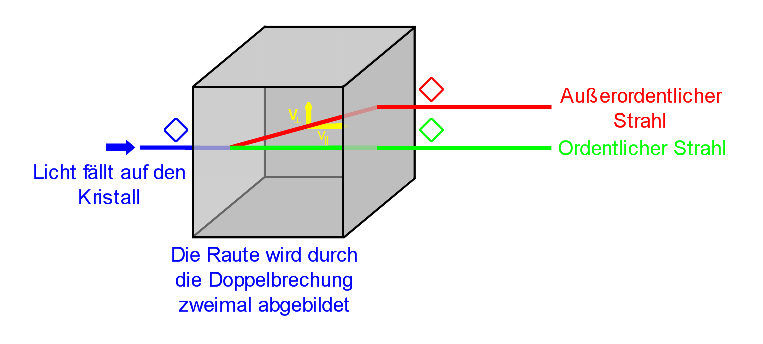
\includegraphics[width=1\linewidth]{pictures/doppelbrechung.eps}
\caption{Doppelbrechung an einem Kristall}
\end{figure}

\subsubsection[Berechnung des linearen elektrooptischen Koeffizienten]{Berechnung des linearen elekrooptischen Koeffizienten für eine ADP-Pockelszelle in $45^\circ$-Y-Cut}
Das Indexellipsoid für einen ADP-Kristall bei einem angelegten elektrischen Feld ist bis zur ersten Ordnung:
\begin{align}
\label{indexellips}
 \frac{x_1^2}{n_1^2} + 2 r_{41} x_2 E_1 x_3 + \frac{x_2^2}{n_1^2} + 2 r_{41} x_1 E_2 x_3 + \frac{x_3^2}{n_3^2} + 2 r_{63} x_1 x_2 E_3 = 1
\end{align}

Die optische Achse im feldfreien Fall ist hier die $x_3$-Achse. Bei Anlegen des elektrischen Feldes entlang der $x_1$-Achse wird (\ref{indexellips}) zu:
\begin{align}
 \frac{x_1^2}{n_1^2} + 2 r_{41} x_2 E_1 x_3 + \frac{x_2^2}{n_1^2} + \frac{x_3^2}{n_3^2} = 1
\end{align}

der Y-Cut: Koordinatenwechsel durch Drehung um $45^\circ$ um die $x_1$-Achse:
\begin{align*}
 \notag x_2 = \frac{1}{\sqrt{2}} (x'_2 + x'_3) \quad x_3 = \frac{1}{\sqrt{2}} (x'_2 - x'_3) \\[10pt] 
 \frac{x_1^2}{n_1^2} + r_{41} ( {x'_2}^2 - {x'_3}^2) E_1 + \frac{(x'_2 + x'_3)^2}{2 n_1^2} + \frac{(x'_2 - x'_3)^2}{2 n_3^2} = 1\\[10pt]
\notag \Leftrightarrow \frac{x_1^2}{n_1^2} + \frac{{x'_2}^2}{2} \left(\frac{1}{n_1^2} + \frac{1}{n_3^2}\right) + \frac{{x'_3}^2}{2} \left(\frac{1}{n_1^2} + \frac{1}{n_3^2}\right) + x'_2 x'_3 \left(\frac{1}{n_1^2} - \frac{1}{n_3^2}\right) + r_{41} E_1 ({x'_2}^2 - {x'_3}^2) = 1 \\[10pt]
\notag \textnormal{mit} \quad \frac{1}{n_x^2} = \frac{1}{2}\left(\frac{1}{n_1^2} + \frac{1}{n_3^2}\right) \\[10pt]
\notag \Leftrightarrow \frac{x_1^2}{n_1^2} + \frac{{x'_2}^2}{n_x^2} + \frac{{x'_3}^2}{n_x^2} + x'_3 x'_3 \left(\frac{1}{n_1^2} - \frac{1}{n_3^2} \right) + r_{41} E_1 ({x'_2}^2 - {x'_3}^2) = 1 \\[10pt]
\notag \Leftrightarrow \frac{x_1^2}{n_1^2} + \frac{{x'_2}^2}{n_x^2} (1 + r_{41} E_1 n_x^2) + \frac{{x'_3}^2}{n_x^2} (1 - r_{41} E_1 n_x^2) + x'_2 x'_3 \left(\frac{1}{n_1^2} - \frac{1}{n_3^2}\right) = 1
\end{align*}

Für den Brechungsindex der jeweiligen Polarisationskomponente bei Lichteinfall entlang der $x'_2 (x'_3)$-Richtung, polarisiert entlang der Winkelhalbierenden zu $x_1$, $x'_3 (x'_2)$, gilt dann:
\begin{align}
 n_{x'_2} = \frac{n_x}{\sqrt{1 + r_{41} E_1 n_x^2}} \approx n_x + \frac{1}{2} r_{41} E_1 n_x^3 \\[10pt]
\notag \left( n_{x'_3} = \frac{n_x}{\sqrt{1 - r_{41} E_1 n_x^2}} \approx n_x - \frac{1}{2} r_{41} E_1 n_x^3 \right)
\end{align}

Die Phasenverschiebung nach Durchlauf durch einen Kristall der Länge $l$ ist dann:
\begin{align}
 \omega~t = \frac{2~\pi}{\lambda}~(n_1 - n_{x'_2})~l
\end{align}

In dem hier verwendeten Aufbau wird wie schon erwähnt unter einem Winkel von $45^\circ$ in den Kristall eingestrahlt. Hierdurch werden natürlich außerordentlicher und ordentlicher Strahl räumlich aufgespalten. Um dies zu kompensieren wird ein Zweiter Kristall nachgeschaltet welcher gerade umgekehrt orientiert ist (also um $180^\circ$ gedreht ist).

Außerdem möchte man nur die durch das Elektrische Feld induzierte Doppelbrechung beobachten, da bei dem Kristall aber auch die natürliche Doppelbrechung auftritt wird ein weiteres Kristallpaar welches um $90^\circ$ gedreht ist nachgeschaltet. Bei diesem Paar ist außerdem das Elektrische Feld gegenüber dem des ersten Paars invertiert um nicht auch den Pockelseffekt zu kompensieren. Die Phasenverschiebung nach diesen vier Kristallen beträgt:
\begin{align}
 \omega~t = \frac{4~\pi}{\lambda}~r_{41}~E_1~n_x^3~l
\end{align}

Und für den elektrooptischen Koeffizienten gilt dann (Phasenverschiebung $= \pi$ und $E = U/d$:
\begin{align}
 r_{41} = \frac{\lambda d}{4 l U_{\frac{\lambda}{2}}} \sqrt{\frac{1}{2} \left( \frac{1}{n_1^2} + \frac{1}{n_3^2}\right)^3}
\end{align}

\begin{figure}[H]
\centering
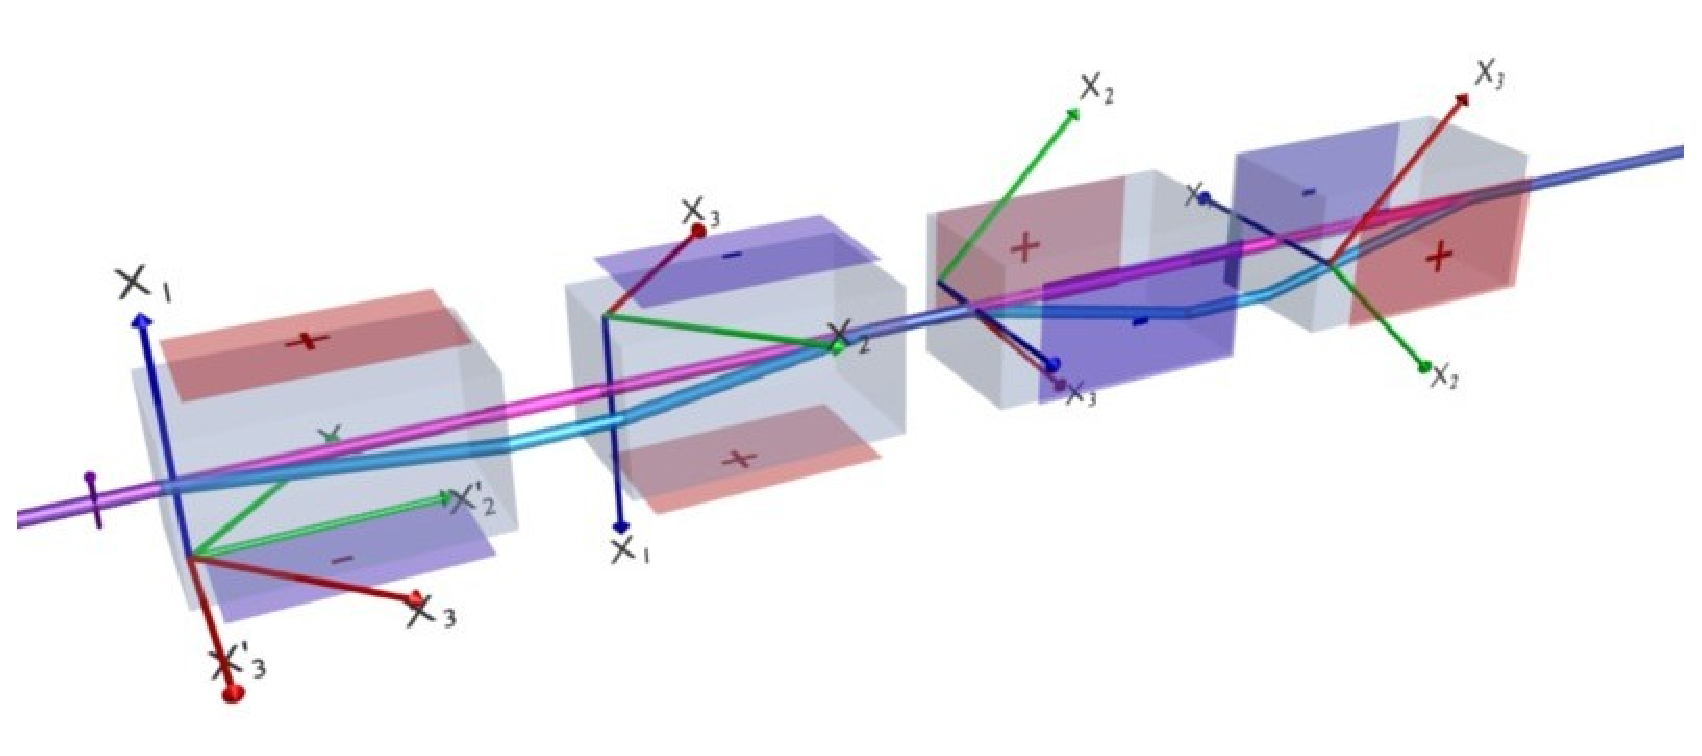
\includegraphics[width=1\linewidth]{pictures/adp-zelle.eps}
\caption{ADP-Pockelszelle mit vier Kristallen}
\end{figure}

Einige Daten über die beim Versuch verwendete Zelle:
\begin{itemize}
 \item Kantenlänge $d \approx 2,4 mm$
 \item Länge $l \approx 20 mm$
 \item $r_{41} = 23,4 \frac{pm}{V}$ bei $21^\circ$C
 \item $n_1 = 1,522$
 \item $n_3 = 1,477$
 \item Laserwellenlänge $\lambda = 632,8 nm$
\end{itemize}

\subsection{Faraday-Effekt}
Der \textbf{Faraday-Effekt} ist ein magneto-optischer Effekt. Er beschreibt die Drehung der Polarisationsebene von polarisiertem Licht beim Durchgang durch ein transparentes Medium, an das ein Magnetfeld parallel zur Ausbreitungsrichtung der Lichtwelle angelegt wurde. Er tritt in den meisten dielektrischen Materialien (einschließlich Flüssigkeiten) auf, wenn sie einem starken magnetischen Feld ausgesetzt werden. Die Drehung der Polarisationsebene ist umso größer, je stärker das angelegte Feld ist.

\begin{figure}[H]
\centering
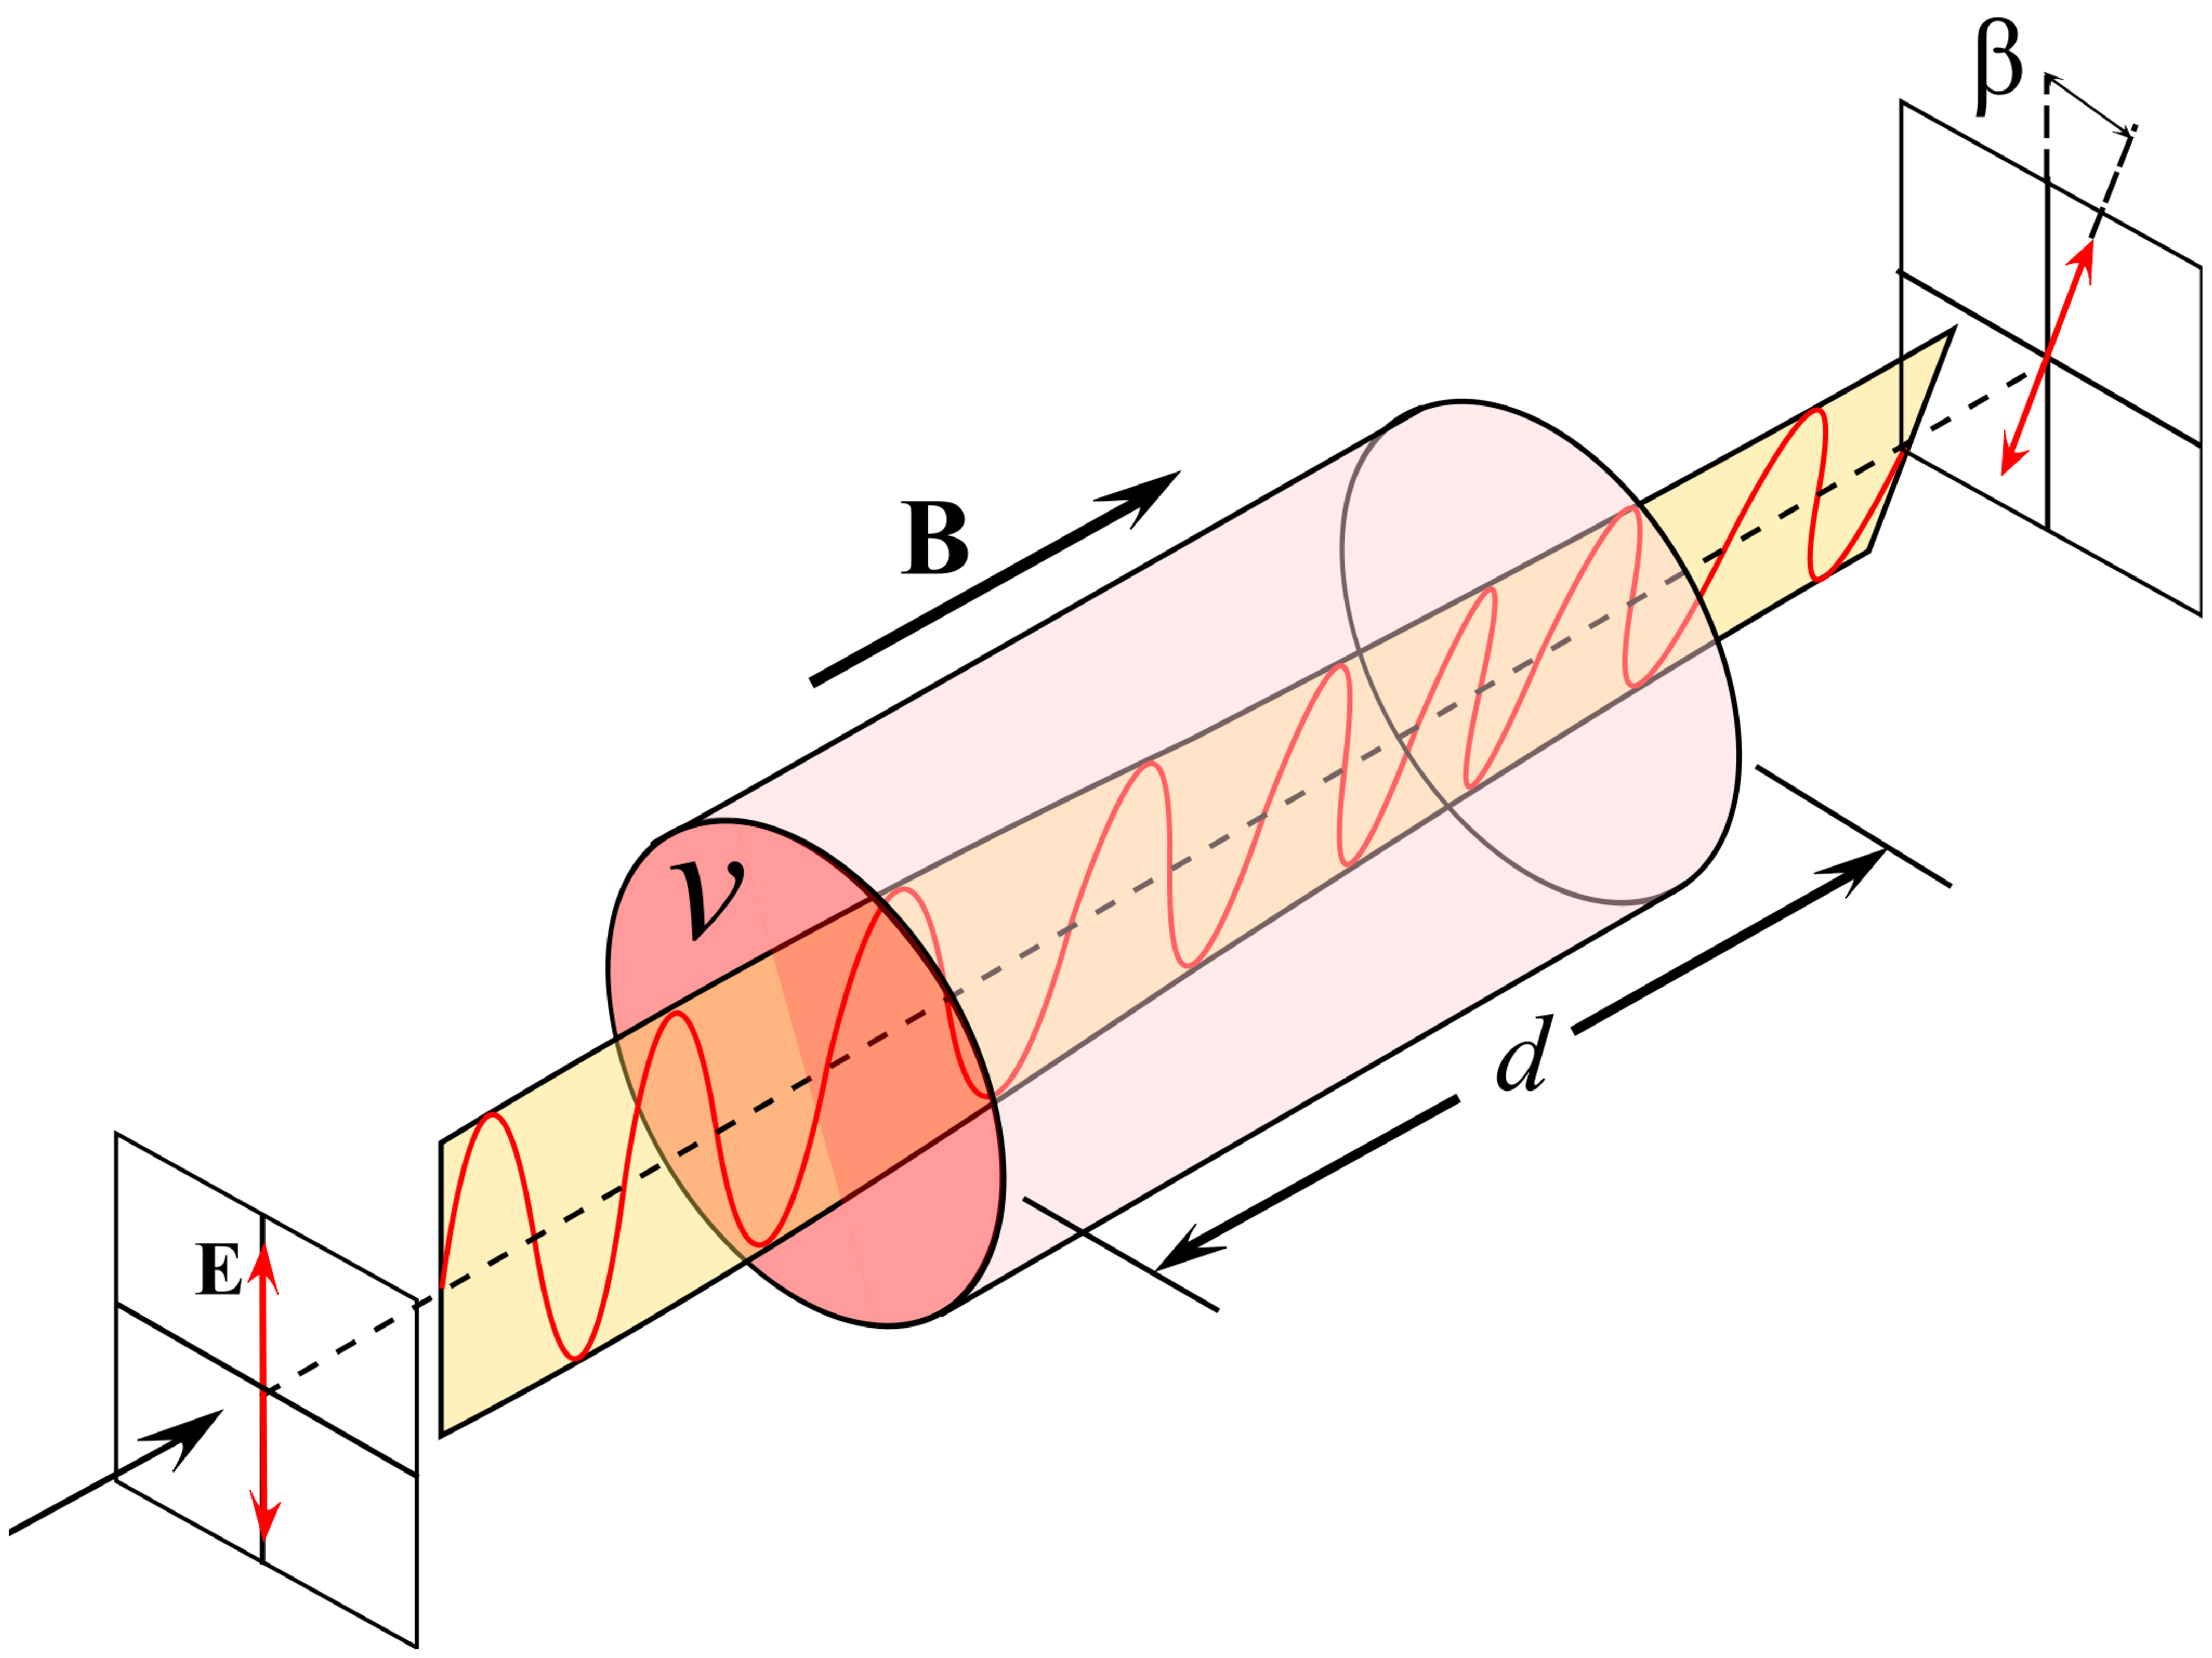
\includegraphics[width=0.8\linewidth]{pictures/faraday-effect.eps}
\caption{Faradayeffekt}
\end{figure}

Die Drehrichtung hängt von der Richtung des Magnetfelds ab. Die Drehung folgt dem Gesetzt:
\begin{align}
 \alpha = V ~ l ~ B
\end{align}

wobei $V$ eine Materialkonstante, die sogenannte Verdetkonstante, $l$ die Länge und $B$ die magnetische Feldstärke ist.
Die Verdetkonstante hängt von der Wellenlänge des verwendeten Lichts ab.

Im Gegensatz zu natürlich drehenden Substanzen hängt der Faraday-Effekt nicht von der Ausbreitungsrichtung im Material ab.
Wenn ein Strahl also das Medium vor und nach Reflexion an einem Spiegel durchläuft wird die Polarisationsrichtung nicht verändert (es wird hin und wieder zurück gedreht).\\

Begründet wird der Faradayeffekt durch die zirkulare Doppelbrechung: Eine einfallende Welle wird in zwei entgegengesetzt zirkular polarisierte Wellen zerlegt. Durch das anliegende Magnetfeld erfahren die beiden Wellen verschiedene Ausbreitungsgeschwindigkeiten. Hierbei ist im Allgemeinen die Welle deren Polarisation mit der Stromrichtung des magnetisierenden Stroms zirkuliert, die mit der schnelleren Ausbreitungsrichtung.
Für die Drehung der Polaristationsebene folgt aus geometrischen Überlegungen:
\begin{align}
 \alpha = \frac{\omega l}{2} \left( \frac{1}{v_-} - \frac{1}{v_+} \right) = \frac{\omega l}{2 c} ( n_- - n_+)
\end{align}

mit $\omega$ Winkelgeschwindigkeit der Welle, $l$ Länge des Mediums, $v_-$ Ausbreitungsgeschwindigkeit der negativ (entgegen $I_B$) zirkulierenden Welle, $v_+$ Ausbreitungsgeschwindigkeit der positiv zirkulierenden Welle und den Brechungsindizies $n_\pm = \frac{c}{v_\pm}$.




\section{Versuchsaufbau}

\subsection{Pockels-Effekt}

Als Lichtquelle dient ein HeNe-Laser. Der Laserstrahl wird durch einen Polarisationsfilter polarisiert bevor dieser auf die Pockelszelle trifft. Nach der Pockelszelle folgt ein weiterer Polarisationsfilter der als Analysator dient. Zur Signalaufnahme trifft der Strahl nach dem Analysator auf eine Photodiode. Das Signal der Photodiode wird nach Verstärkung auf einem Oszilloskop angezeigt.

Für die Spannung an der Pockelszelle steht entweder eine Sägezahnspannung ($0 - 500V$) oder eine Sinusspannung (ca. $40V_{pp}$), welcher eine Gleichspannung ($-300~-~+300V$) überlagert werden kann, zur Verfügung. Die Spannung kann jeweils auch auf dem Oszilloskop beobachtet werden (Bei Sägezahn über Spannungsteiler).

\begin{figure}[H]
\centering
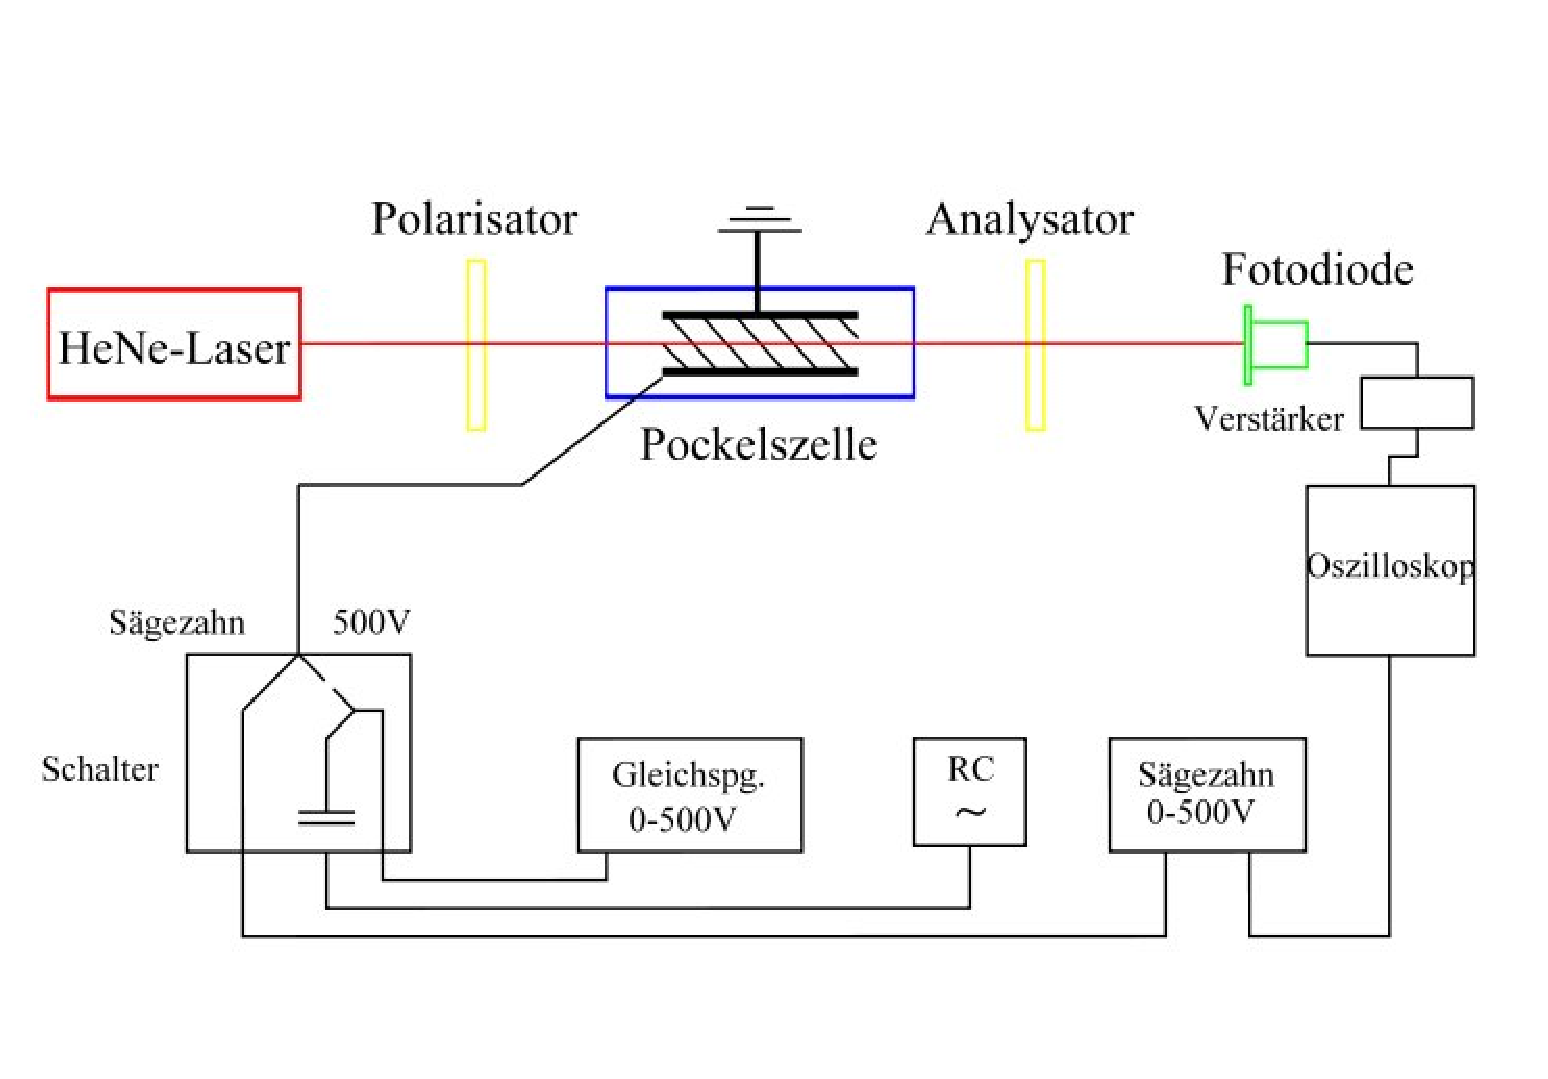
\includegraphics[width=0.9\linewidth]{pictures/aufbau-pockels.eps}
\caption{Schema Versuchsaufbau Pockelseffekt}
\end{figure}

\subsection{Faraday-Effekt}

Das für den Faraday verwendete Schwerflintglas befindet sich in einem Halbschattenpolarimeter welches von einer Spule umwickelt ist. Als Lichtquelle dient eine Natriumdampflampe. Zum Betrieb der Spule steht ein Netzteil zur Verfügung ( $-5~-~+5A$ durch Umpolen).

\begin{figure}[H]
\centering
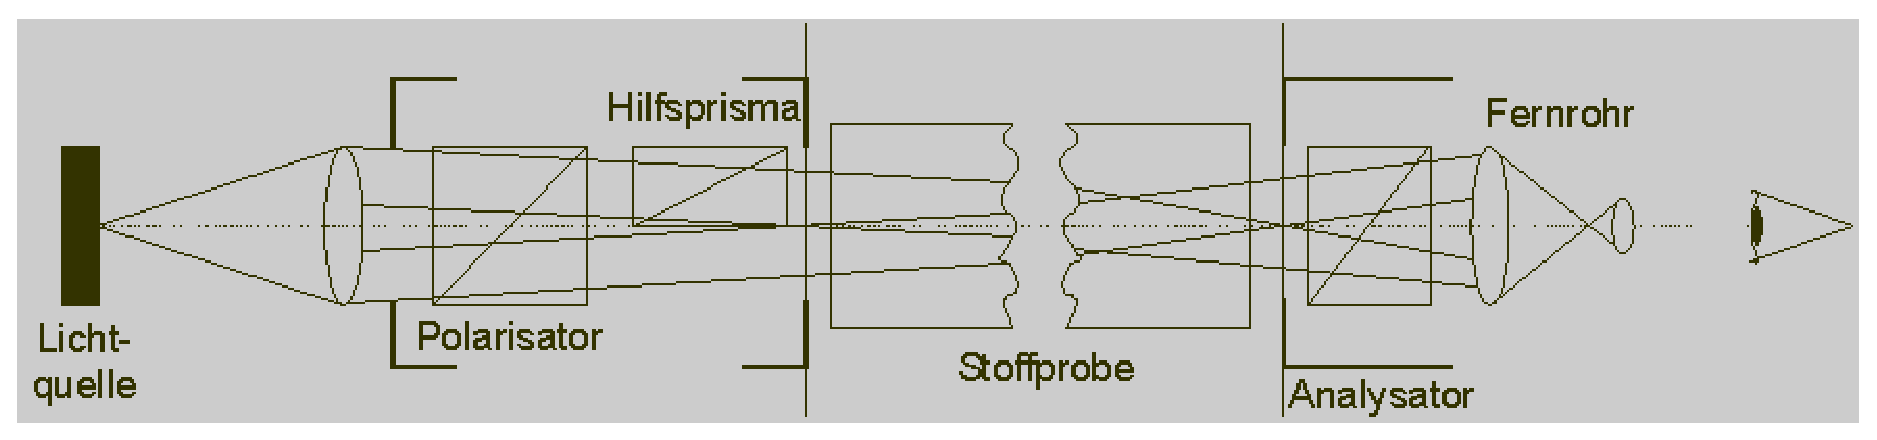
\includegraphics[width=1\linewidth]{pictures/halbschattenpolarimeter.eps}
\caption{Schema Halbschattenpolarimeter}
\end{figure}


\section{Durchführung}
\subsection{Pockels-Effekt}
Nachdem wir uns vergewissert hatten, dass die Optik korrekt justiert war, begannen wir mit der Sägezahnmethode.
Wir stellten die Schalterstelltung am Auswahlschalter auf Sägezahn und führten vier Messungen durch. Die Spannungswerte wurden am PC mit der Oszilloskopsoftware abgelesen.

Wir bestimmten den Teilungsfaktor des Spannungsteiler durch Anschluss der Sinusspannung direkt ans Oszilloskop und mit Spannungsteiler.

Im Sinus-Gleichspannungsmodus nahmen wir jeweils abwechselnd Maximum und Minimum auf. Wir nahmen jeweils 15 Messpunkte auf.

\subsection{Faraday-Effekt}
Nach einschalten der Spulenkühlung und der Lampe begannen wir mit der Messung.
Wir führten zwei Messreihen von jeweils $-5$ bis $+5A$ in $0,5A$ Schritten durch. Hierbei haben wir den Winkel stets auf beiden Seiten der Anzeige abgelesen. Außerdem bestimmten wir den $2\epsilon$-Winkel des Polarimeters (Winkel zwischen den beiden Polarisationsrichtungen).


\section{Auswertung}
Für die genauen Berechnungen siehe Anhang.

\subsection{Pockels-Effekt}
Für den Teilungsfaktor des Spannungsteiler erhielten wir $108,64$.
Bei der Messung mit Sägezahnmethode Berechnet sich der Mittelwert für die Halbwellenspannung $U_{\lambda / 2}$ zu: $(248,79 \pm 3,89)V$. Für die Messung mit der Sinus-Gleichspannungs-Überlagerung erhält man im Mittel $U_{\lambda /2} = (246,93 \pm 1,20)V$.\\

Das Gewichtete Mittel aus diesen beiden Messreihen ergibt sich somit zu: 
\begin{align*}
 U_{\lambda / 2} = (247,37 \pm 0,92)V
\end{align*}

Somit errechnet sich der elektrooptische Koeffizient zu:
\begin{align*}
 r_{41} = (32,22 \pm 0,19) \frac{pm}{V}
\end{align*}


\subsection{Faraday-Effekt}
Wir müssen die Abhängigkeit zwischen Magnetfeldstärke und Spule berechnen. Die Berechnung erfolgt mittels Biot-Savart und lässt sich in der Staatsexamensarbeit nachlesen. Hier nur soviel:
Das Magnetfeld auf der $z$-Achse berechnet sich durch Integration von
\begin{align}
 dH = \frac{1}{4\pi}\frac{I~dl}{r^2} \sin(\phi)
\end{align}
zu
\begin{align}
 H(z) = \frac{NI}{2L(x_2-x_1}\left((L-z)\ln\frac{x_2 + \sqrt{(L-z)^2 + x_2^2}}{x_1 + \sqrt{(L-z)^2 + x_1^2}} + z \ln \frac{x_2 + \sqrt{z^2 + x_2^2}}{x_1 + \sqrt{z^2 + x_1^2}}\right)
\end{align}

Setzt man z.B. $1A$ ein so erhält man in der Mitte der Spule:
\begin{align}
 H\left(\frac{L}{2}\right) = 8212 \frac{A}{m}
\end{align}

Würde man mit der Näherung für eine undenlich lange Spule rechnen so erhielte man:
\begin{align}
 H\left(\frac{L}{2}\right) = 20571 \frac{A}{m}
\end{align}

Wir rechnen also mit der exakten Formel.

Um den Rotationswinkel zu erhalten muss man erneut Integrieren, auch hier sei wieder auf die Staatsexamensarbeit verwiesen.
\begin{align}
 d\alpha = V H(z) dz \Leftrightarrow \alpha = V \int\limits_{\frac{L-l}{2}}^{\frac{L-l}{2}} H(z) dz
\end{align}
wird zu:
\begin{align}
 \alpha = V I 2556 \quad \textnormal{bzw.} \quad V = \frac{\alpha}{I 2556}
\end{align}

\begin{figure}[H]
\centering
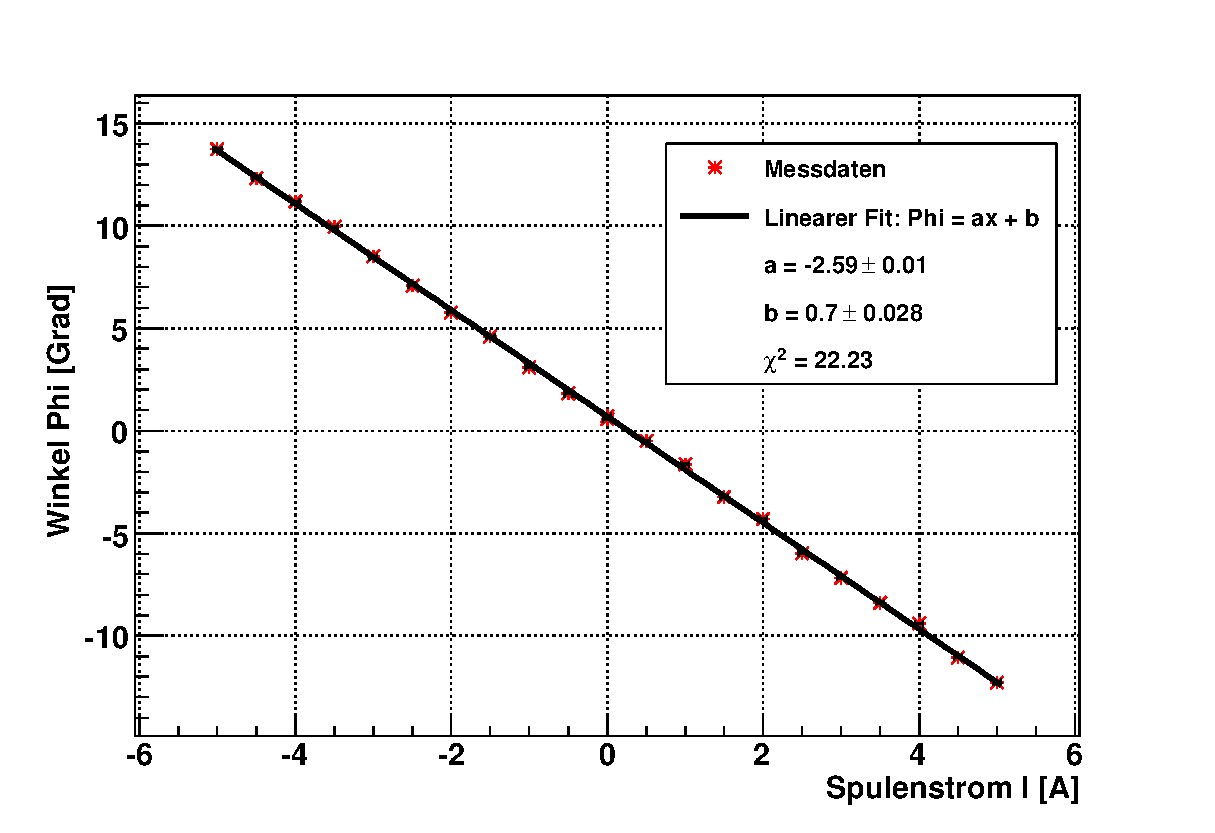
\includegraphics[width=0.9\linewidth]{pictures/faraday.eps}
\caption{Plot mit Fit der Messung des Faradayeffekts}
\end{figure}

Wir teilen also die aus dem Fit erhaltene Steigung durch $2556$ um die Verdetkonstante zu erhalten.
\begin{align}
 V =  1,02 \cdot 10^-3 \frac{^\circ}{A}
\end{align}

Dies lässt sich umrechnen um mit den Herstellerangaben vergleichen zu können:
\begin{align}
 V = 1,02 \cdot 10^{-3} \frac{60min}{1,2564Oe~cm} = 0,485 \frac{min}{Oe~cm}
\end{align}

Ohne das Magnetfeld im Inneren der Spule tatsächlich zu vermessen ist sicherlich der Fehler auf das Magnetfeld der führende.
Eine Fehlerabschätzung macht in diesem Versuchsteil also wenig Sinn weshalb auch auf eine solche verzichtet wurde.

Für den $2\epsilon$-Winkel des Polarimeters haben wir $13,4 \pm 0,15^\circ$ gemessen.

\section{Zusammenfassung}
Für den elektrooptischen Koeffizienten beim Pockelseffekt erhielten wir:
\begin{align*}
 r_{41} = (32,22 \pm 0,19) \frac{pm}{V}
\end{align*}

Der angegebene Literaturwert beträgt $24,4 \frac{pm}{V}$ bei $21^\circ$. Eine Temperaturmessung stand uns leider nicht zur Verfügung, auch die Literaturangabe zur Temperaturabhängigkeit steht nicht zur Verfügung. Es lässt sich somit nur sagen das der von uns gemessene Wert in der richtigen Größenordnung liegt.\\

Bei Faradayeffekt erhielten wir für die Verdetkonstante:
\begin{align}
 V =  1,02 \cdot 10^-3 \frac{^\circ}{A}
\end{align}
bzw.
\begin{align}
 V = 0,485 \frac{min}{Oe~cm}
\end{align}

Der Literaturwert liegt bei $0,05 \frac{min}{Oe~cm}$. Da wie schon erwähnt keine Fehlerabschätzung durchgeführt wurde lässt sich hier ebenso nur die Aussage über die richtige Größenordnung treffen.

\section{Anhang}
\subsection{Programmausgabe}
\lstinputlisting[language=python]{../plot/farpock.out}
\subsection{Quelltext}

\lstinputlisting[language=python]{../plot/farpock.py}

\end{document}
